% Created 2023-02-07 Tue 13:51
% Intended LaTeX compiler: xelatex
\documentclass[presentation]{beamer}
\usepackage{graphicx}
\usepackage{longtable}
\usepackage{wrapfig}
\usepackage{rotating}
\usepackage[normalem]{ulem}
\usepackage{amsmath}
\usepackage{amssymb}
\usepackage{capt-of}
\usepackage{hyperref}
\usepackage[scheme=plain]{ctex}
\usetheme{boxes}
\author{Jinghui Hu}
\date{\textit{<2023-02-07 Tue 13:41>}}
\title{MacOS 工具}
\hypersetup{
 pdfauthor={Jinghui Hu},
 pdftitle={MacOS 工具},
 pdfkeywords={},
 pdfsubject={},
 pdfcreator={Emacs 28.2 (Org mode 9.5.5)},
 pdflang={English}}
\begin{document}

\maketitle
\begin{frame}{Outline}
\tableofcontents
\end{frame}


\begin{frame}[label={sec:org69b32f3}]{桌面美化}
\begin{block}{时钟屏保 fliqlo}
\begin{enumerate}
\item \href{https://fliqlo.com/screensaver/}{Download} | \href{https://www.xiaohongshu.com/explore/62f22988000000001200fdab}{安装教程}
\item 替换项目 \href{https://github.com/phaselden/FlipIt}{Fliplt}
\end{enumerate}

\begin{center}
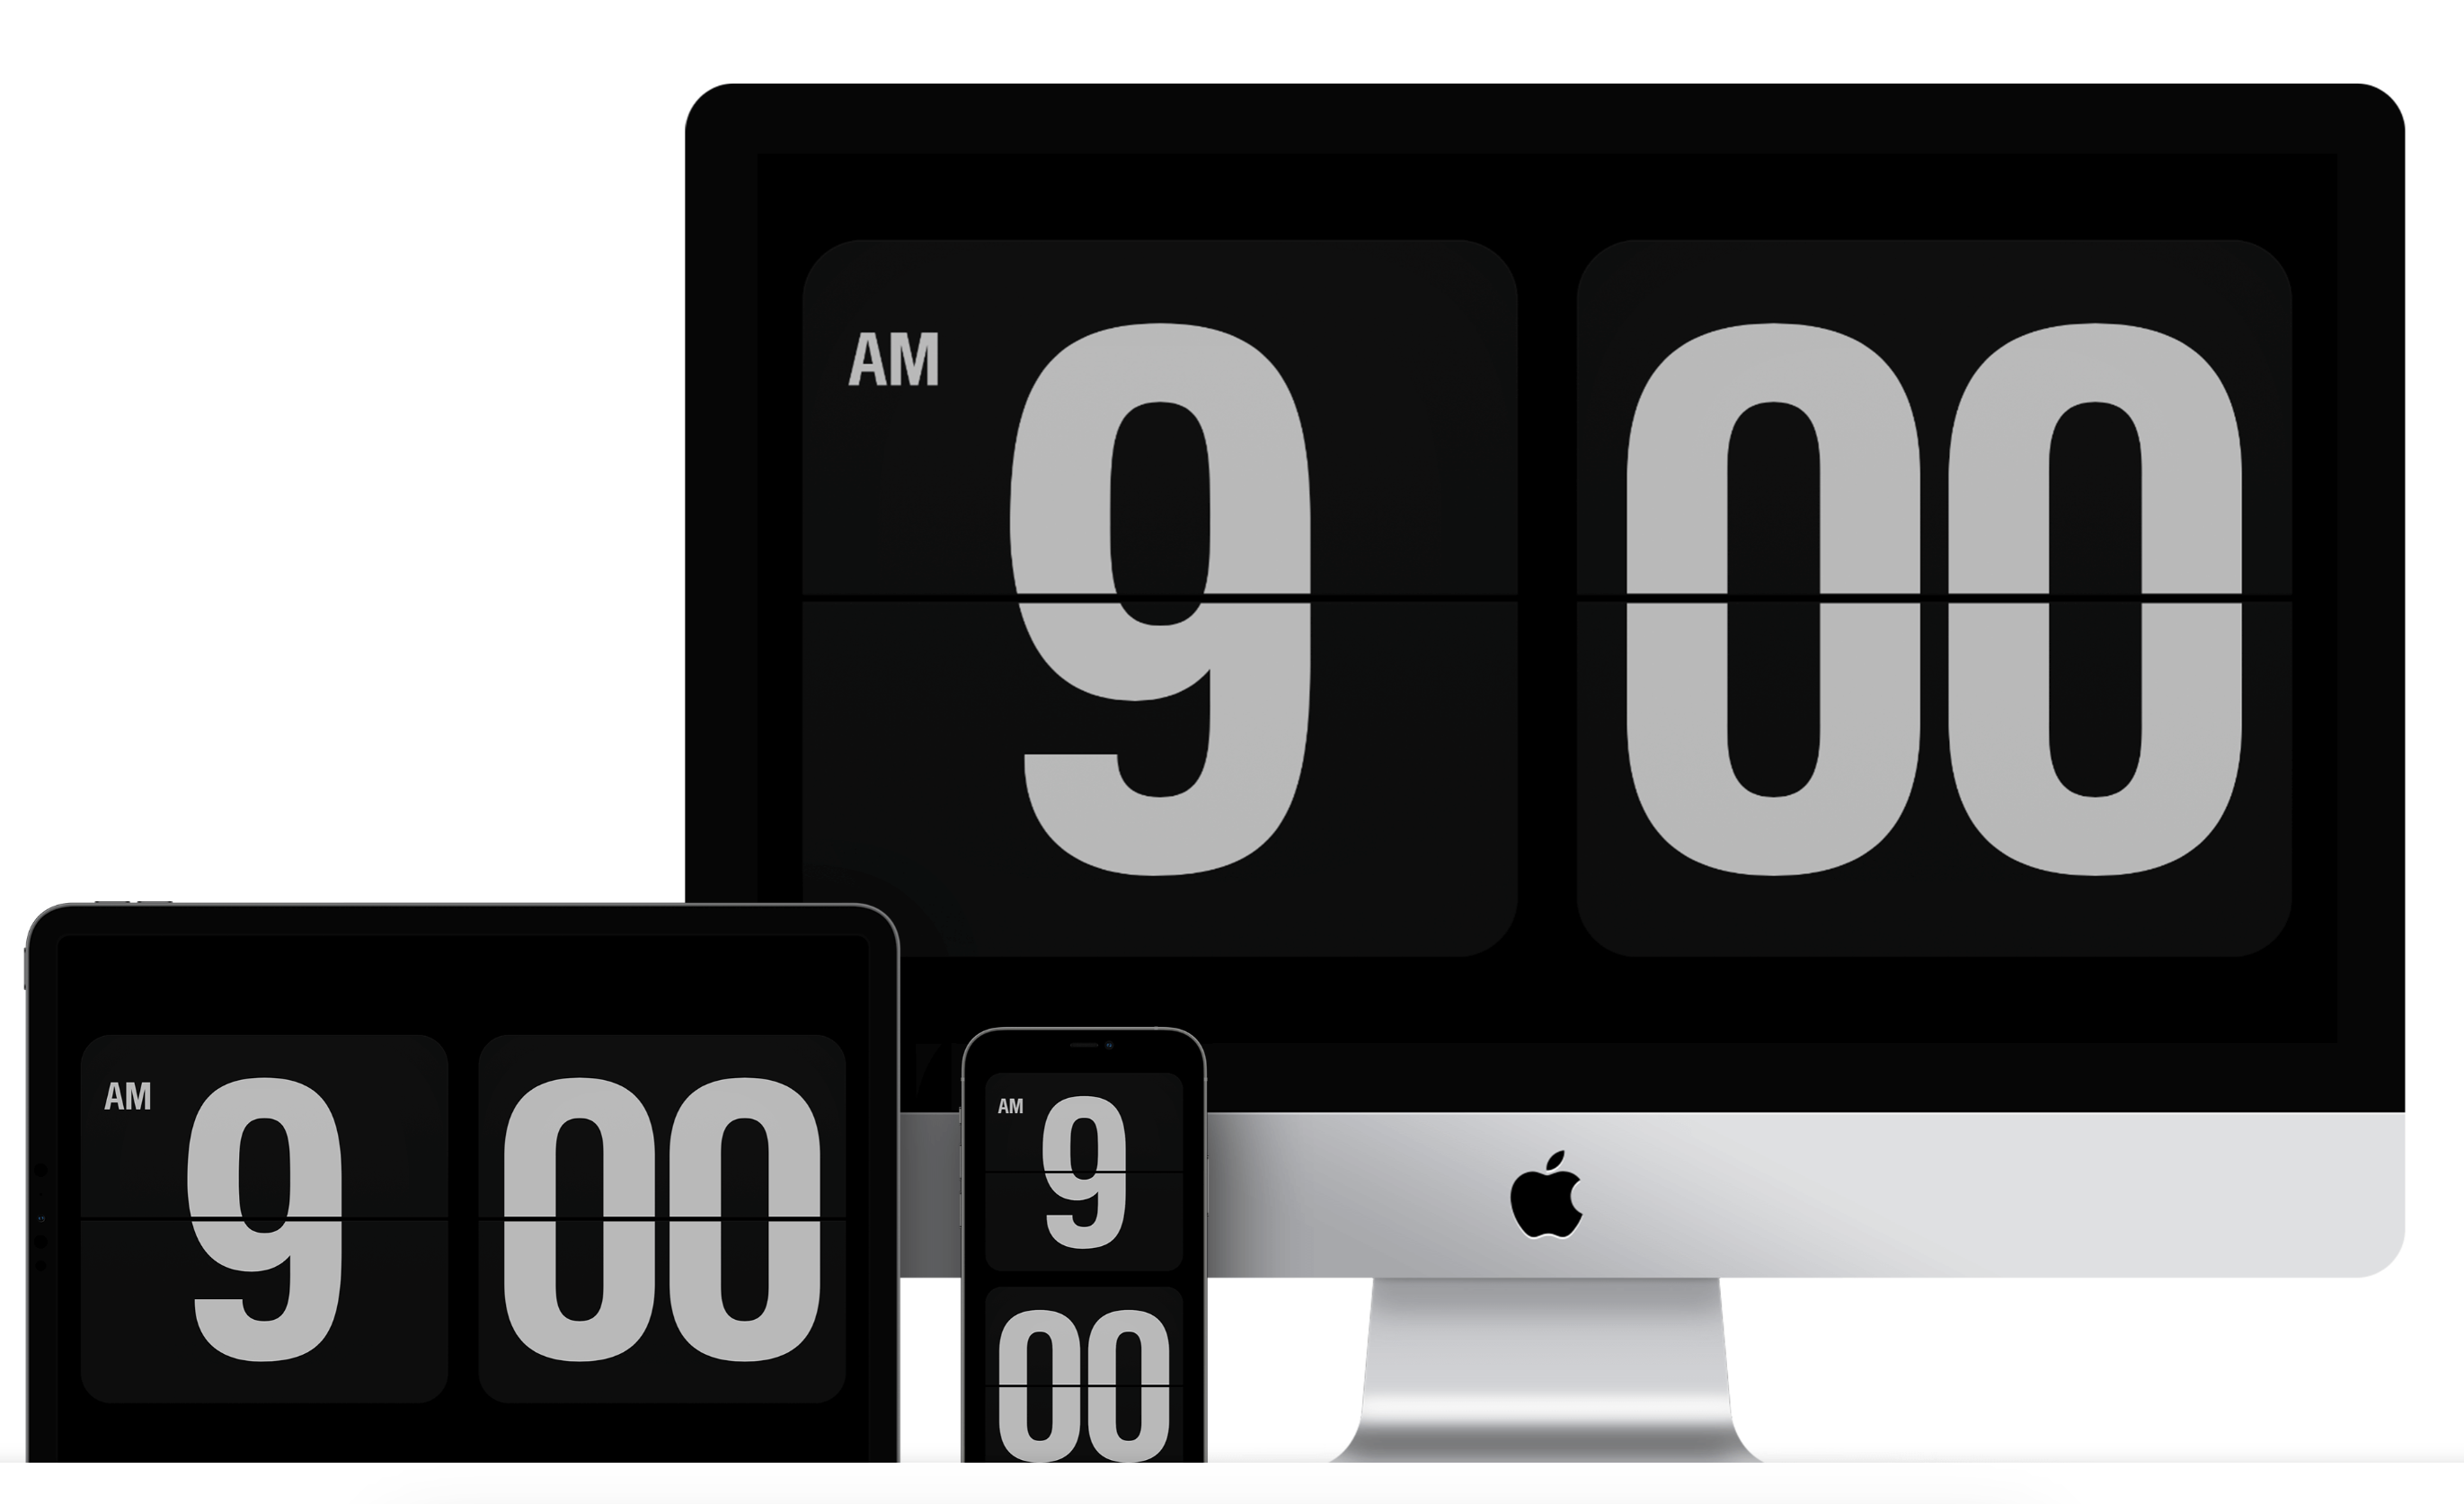
\includegraphics[width=.9\linewidth]{../static/image/2023/0207/134403.png}
\end{center}
\end{block}
\end{frame}

\begin{frame}[label={sec:org0a6d636}]{开发工具}
\end{frame}

\begin{frame}[label={sec:org336bd6e}]{系统问题}
\end{frame}
\end{document}